%% main.tex
%% V1.4
%% 2019/12/18
%% by Anthony Escalona

\documentclass[conference]{IEEEtran}
\usepackage{times}
\usepackage{epsfig}
\usepackage[numbers,sort&compress]{natbib}
\usepackage[protrusion=true,expansion=true]{microtype}              % Better 
\usepackage{multirow}
\usepackage{multicol}
\usepackage{rotating}
\usepackage{setspace}
%\usepackage{mdwlist}
\usepackage{comment}
\usepackage{color}                  
%\label{\label{key}}     % To highlight changes by author
\usepackage{xspace}
\usepackage{dcolumn} % used to correctly align numbers in tables
\usepackage[noorphans,font=itshape]{quoting}
\usepackage[english]{babel}

\setlength{\parindent}{2em}
\setlength{\parskip}{0em}
\renewcommand{\baselinestretch}{1}
\onehalfspacing

%This is used with dcolumn.sty. Defines the "." to be the line up character.
\newcolumntype{.}{D{.}{.}{2}}
\newcolumntype{f}{D{.}{.}{2}}
\newcolumntype{d}{D{.}{.}{0}}

\begin{document}
%
% paper title
% can use linebreaks \\ within to get better formatting as desired
% Do not put math or special symbols in the title.
\title{Cloud Data Platform for the Lifecycle Management of Data Analytics (Proposal) }


% author names and affiliations
% use a multiple column layout for up to three different
% affiliations
\author{\IEEEauthorblockN{Anthony Escalona}
	\IEEEauthorblockA{\textit{Pace University}\\
		\textit{Seidenberg School of CSIS} \\
		New York, NY 10038 \\
		ae50483p@pace.edu}
	\and
	\IEEEauthorblockN{Felipe Flores}
	\IEEEauthorblockA{\textit{City of New York}\\
		\textit{DOITT} \\
		Brooklyn, NY 11201 \\
		fflores@doitt.nyc.gov}

}

% make the title area
\maketitle{}

% As a general rule, do not put math, special symbols or citations
% in the abstract
\begin{abstract}
Software development is becoming a mammoth task with the introduction of Big Data and Analytics and the programming languages they use, along with data processing, creation, preparation,  and modeling operations.  Furthermore, with a plethora of cloud-based data management platforms, heterogeneity in hardware, increased focus on exploiting edge computing resources for low-latency prediction serving and often a lack of a complete understanding of resources required to execute workflows efficiently, data deployment demands expertise for managing the lifecycle of data workflows efficiently and with minimal cost. Also, with the proliferation of cloud based data management systems, hardware complexity, increased emphasis on using cutting-edge computing resources to support fast feedback and often a lack of comprehensive understanding of the resources needed to effectively execute workflows, data implementation needs expertise to handle the lifecycle of data workflows efficiently and with a minimum set of cost.  This paper describes the AWS SageMaker platform highlighting the problems it resolves.

\end{abstract}
\section{Introduction}
In data science, writing code for data loading, transformation and pre-processing, and choosing the right algorithm for analyzing the data and then evaluating the model requires expertise.  Data Analytics continues to be one of the most effective data-driven approaches for using big data to improve processes and decision making, but integrating data workflows and pipelines into existing data environments remains a challenge. It isn't straightforward to prepare data for data pipelines if end-to-end software and analytical systems are not optimized to interoperate with existing analytical platforms. New design concepts can help, but to apply them appropriately, software engineers must understand end-to-end workflows.  Agencies are trying to operationalize information pipelines to support large data projects in development, but are struggling to establish effective strategies for operations and best practices.  Agencies are strengthening the division of duties among data/big data engineers, software engineers, data scientists, and the data architect role to accelerate the delivery of big data projects. 

The right cloud platform configurations can enhance performance and minimize cost, which is generally lacking in data developers. According to EMC\cite{EMC}, the requirements for Data Analytics Lifecycle Management is broken down into six phases. 1) Discovery, 2) Data Prep, 3) Model Planning, 4) Model Building, 5) Communicate Results, and 6) Operationalize.

To that end, we propose using machine learning (ML) platform by AWS called SageMaker\cite{SageMaker}, which addresses the management lifecycle challenges of data analytics in a cloud centric environment.  The rest of this paper, we present the M otivation in Section II, the Problem Statement and Justification in Sections III and IV, and Objectives.
%
%
%
\section{Motivation}
Exploring the opportunities that big data presents require new data architectures,  new ways of working, and people with unique skill sets. The authors are motivated to identify and understand the socio-cultural, organizational, process, and technology challenges that public agencies face in designing and implementing a digital platform.  

Establishing a vision to serve citizens better and inspire civil servants will require the ability to rethink processes in a cross-functional way, while research suggests that it has proven difficult in government entities\cite{Weerakkody}.  Importantly, we intend to focus not on understanding today's processes but instead shaping tomorrow's processes. The common theme behind this transformation involves automation or computerization of existing methods that will prompt new ways of debating and deciding strategies, new ways of listening to citizens and communities, and new ways of organizing and delivering information\cite{eGov} through a data platform.  

A data analytic lifecycle platform can help agencies in a variety of ways, including solving Big Data problems and data science projects. It allows them to aggregate and analyze data from across local agencies to more effectively address crime, public safety, and quality of life issues. 
%
%
\section{Problem Statement}
Big data analytics continues to be one of the most effective data-driven approaches for using big data to improve processes and decision making, but integrating data workflows and pipelines into existing data environments remains a challenge. Automation can help.  Many organizations are looking to operationalize data pipelines to support their big data initiatives in production, but struggle to build effective strategies and best practices. We seek to strengthen the division of duties among data engineers, software engineers, data scientists, and data architect roles to accelerate the delivery of data.


\section{Justification}
Establishing a data lifecycle management creates a fast flow of work as it moves from discovery to operationalization.  Significantly, it shortens and amplifies the feedback loop to address data issues early and often for data engineer practitioners.  By definition, a data engineer executes the actual data extractions and performs substantial data manipulation to facilitate the analytics.  In turn, they work closely with the data scientist to help shape data in the right ways for analyses.  A common data pipeline platform help facilitate and ensures that data is clean, organized, and presentable.

Practitioners often overlap with other people during the data lifecycle. Figure \ref{fig:sdlc}\cite{gartner} describes the data science life cycle, with a responsibility assignment matrix associated with it.  Building and operating an end-to-end data platform requires stakeholders comprised of business subject matter experts, data scientists, and data engineers. However, data preparation, modeling, and evaluation often strain the data scientist, typically resulting in a slow, inconsistent, and mostly manual process for developing ML models.  An expansion of the existing data life cycle is needed to improve inefficiencies and interaction among practitioners related to data development.

\begin{figure}[bth]
	\centering
	\scalebox{.5}{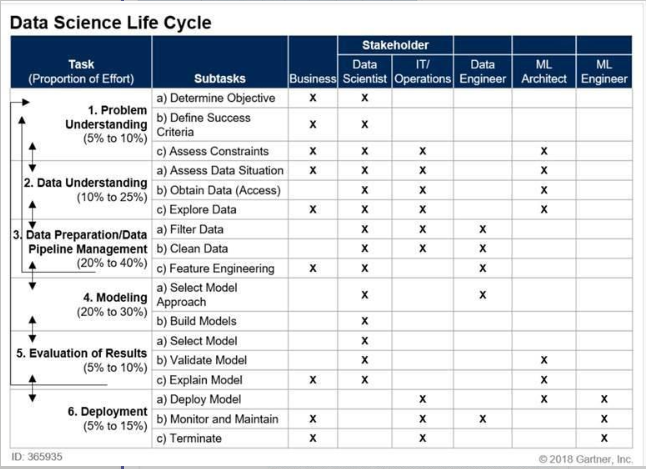
\includegraphics{../figures/dataLifecycle.png}}
	\caption{Gartner}
	\label{fig:sdlc}
\end{figure}

We want to develop this system that will run on the cloud, unlike the current manual system across local agencies. So this system is aimed to solve this entire problem by enabling practitioners to solve business problems quickly, acquire data, process data, model data, communicate results, and deploying data.

\section{Objectives}
Data from a variety of potential sources, such as applications, sensors, networks, and devices, is fed to the system. This system uses that data moves forward and backward as new information is uncovered, and data practitioners learn more about various stages of the data lifecycle.  This enables them to move iteratively through the process and drive toward operationalizing the work.  The result of this study will be valuable to industry practitioners in developing better practices and tools for data management.



% use section* for acknowledgement
\section*{Acknowledgment}
We offer our sincerest gratitude to Al Frangella, Omari Holtz, and Dr. Tappert for supporting this research and reviewing the paper.


\bibliographystyle{IEEEtran}
{\small\bibliography{references}}
 

\end{document}


